%Tipo de documento
\documentclass{beamer}
%Tema
\usetheme{Madrid}
%Color del texto en título
\definecolor{UBCblue}{rgb}{0.6,0.6,0.6} % UBC Blue (primary)0.37, 0.15, 0.10
%Color del encabezado
\definecolor{ColorUNFV}{rgb}{0.37,0.15,0.10} % UBC Blue (primary)

\usecolortheme[named=UBCblue]{structure}
\useinnertheme{circles}
\setbeamercolor{titlelike}{parent=structure,bg=ColorUNFV}

\addtobeamertemplate{footnote}{\vspace{-6pt}\advance\hsize-0.5cm}{\vspace{6pt}}
\makeatletter
% Alternative A: footnote rule
\renewcommand*{\footnoterule}{\kern -3pt \hrule \@width 2in \kern 8.6pt}
% Alternative B: no footnote rule
% \renewcommand*{\footnoterule}{\kern 6pt}
\makeatother

\usepackage[utf8]{inputenc} % Required for inserting images
\usepackage{amsmath}
\usepackage[spanish]{babel}
\decimalpoint
\usepackage{listings}
\usepackage{hyperref}
\usepackage{tikz}
\usepackage{pgfplots}
\tikzset{declare function = {
    H(\x,\y)=(\x)*(\x)*(\x)*(\x)+(\y)*(\y)*(\y)*(\y)-\x;
    acosh(\x)=ln(\x + sqrt(\x-1)*sqrt(\x+1));}}
\usepackage[beamer]{ragged2e}
\usepackage[style=apa,autocite=footnote]{biblatex}
\usepackage{csquotes}
\usepackage{enumitem}
\usepackage{xcolor}
\usepackage{caption}
\newcounter{nameOfYourChoice}


\addbibresource{Referencias1.bib}
\DeclareMathOperator{\acosh}{acosh}
\usepackage{filecontents}
\pgfplotsset{compat=newest}

\titlegraphic { 
\begin{tikzpicture}[overlay,remember picture]
    \node[left=0.2cm] at (current page.335){
        
\includegraphics[width=2cm]{Imagenes/FIC.jpeg}
    };
    \node[right=0.2cm] at (current page.207){
        
\includegraphics[width=2cm]{Imagenes/UNFV.png}
    };

\end{tikzpicture}
}

\title[GRUPO DE ESTRUCTURAS]{GRUPO DE INVESTIGACIÓN DE ESTRUCTURAS\\ 
Tercer avance: Simulación Numérica en Ingeniería 1-3}
\author[Gustavo Delgado]{GUSTAVO IVÁN DELGADO ROMERO}
\institute[UNFV-FIC]{
  \inst{}%
  Facultad de Ingeniería Civil\\
  Universidad Nacional Federico Villarreal
}
\date{Marzo 2024}

\begin{document}

\begin{frame}
    \titlepage 
\end{frame}

\begin{frame}{Contenido}
    \tableofcontents[hideallsubsections]
\end{frame}

\section{Introducción}
\begin{frame}{Introducción}
    \justify
    
    El presente trabajo tiene como finalidad resumir los tres primeros capítulos
    del curso de Master ofrecido por ANSYS en Simulación Numérica en Ingeniería.
    En ese sentido es importante agregar que estos tres primers capítulos cubren
    3 aspectos:
    \begin{itemize}
        \item Prefacio.
        \item Diseño y Optimización de Ingeniería.
        \item Métodos de optimización del tipo gradiente.
    \end{itemize}
\end{frame}
\section{Prefacio}
    %No voy a detenerme en el prefacio, pero sí voy a hacer algunas apreciaciones.
    \begin{frame}{Prefacio}
        El objetivo del curso en general es ofrecer las herramientas necesarias
        a los ingenieros para afrontar problemas de optimización,
        para esto los autores tuvieron a bien enseñar primero los métodos de 
        optimización existentes y finalmente los métodos de diseño de una función
        objetivo susceptible de ser optimizada.
    \end{frame}
\section{Diseño y optimización de Ingeniería}
    \begin{frame}{Diseño y optimización de Ingeniería}
        \tableofcontents[sections={3}]
    \end{frame}
    \subsection{Formulaciones básicas}
        \begin{frame}{Formulaciones básicas}
            Sea el vector $\vec{x}=(x_{1}, x_{2},...x_{N}) $\\
            Lo que buscamos es: $\min F(x_{1}, x_{2},...x_{N}) \equiv \min F(\vec{x})$\\
            Hasta aquí tenemos una función, sin restricciones, pero 
            supongamos que estas variables sometidas a un grupo $m$ de funciones
            $R$ se comporta de manera constante, y estas mismas variables
            sometidas a un grupo $n-m$, con $m<n$ de funciones $R$ arroja resultados 
            dentro de un intervalo dado, es decir:
            $$R_{k}(\vec{x})=0, \text{ para: } k=1,2...m$$
            $$R_{k}(\vec{x})\geq 0, \text{ para: } k=m+1,m+2...n$$
            Lo cual convierte nuestra función objetivo en una función restringida.

        \end{frame}
        \begin{frame}{Formulaciones básicas}
            \begin{figure}[h]
                \centering
                \captionsetup{justification=centering}
                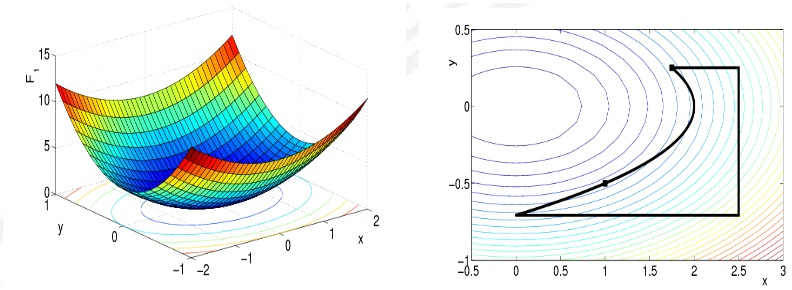
\includegraphics[width=10cm]{Imagenes/Funciones convexas.jpg}
                \caption{Funciones convexas, 
                Izquierda Función sin restricciones, 
                derecha función restringida}
                \centering
            \end{figure}
        \end{frame}

    \subsection{Formulaciones de complejidad incrementada}
        \begin{frame}{Formulaciones de complejidad incrementada}
            Consideremos ahora que algunas de estas variables involucradas
            toman valores fijos, a estas variables fijas las denominaremos parámetros.
            Es así que nuestra formulación básica queda de la siguiente manera:
            Sean el vector $\vec{x}=(x_{1}, x_{2},...x_{n}) $\\
            Y el vector $\vec{p}=(p_{1}, p_{2},...p_{m}) $\\
            Nuestras funciones serían ahora:
            $$F=F(\vec{x},\vec{p})$$
            $$R_{k}=R_{k}(\vec{x},\vec{p})$$
        \end{frame}
        \begin{frame}{Formulaciones de complejidad incrementada}
            Otro escenario posible es que exista un grupo de variables $q$
            que participen de nuestra función objetivo pero que dependen de $x$\\
            Entonces,sea el vector $\vec{x}=(x_{1}, x_{2},...x_{n}) $\\
            Y el vector $\vec{q}=(q_{1}, q_{2},...q_{m}) $\\
            Nuestras funciones serían ahora:
            $$F=F(\vec{x},\vec{q})$$
            $$R_{k}=R_{k}(\vec{x},\vec{q})$$
        \end{frame}
        \begin{frame}{Formulaciones de complejidad incrementada}
            Otro escenario posible es que exista un grupo de variables $y$
            que participen de nuestra función objetivo pero cuyo
            comportamiento sea discreto.\\
            Entonces, sea el vector $\vec{x}=(x_{1}, x_{2},...x_{n}) $\\
            Y el vector $\vec{y}=(y_{1}, y_{2},...y_{m}) $\\
            Nuestras funciones serían ahora:
            $$F=F(\vec{x},\vec{y})$$
            $$R_{k}=R_{k}(\vec{x},\vec{y})$$
        \end{frame}
        \begin{frame}{Formulaciones de complejidad incrementada}
            Finalmente para realizar los análisis de optimización existen los siguientes 
            métodos.
            \begin{itemize}
                \item Métodos del tipo gradiente.
                \item Métodos de búsqueda directa.
                \item Métodos Heurísticos.
            \end{itemize}
        \end{frame}      
\section{Métodos de optimización tipo-gradiente}
    \begin{frame}{Métodos de optimización tipo-gradiente}
        \tableofcontents[sections={4}]
    \end{frame}
    \subsection{Optimización no restringida}
        \begin{frame}{Optimización no restringida}
            \begin{figure}[h]
                \centering
                \captionsetup{justification=centering}
                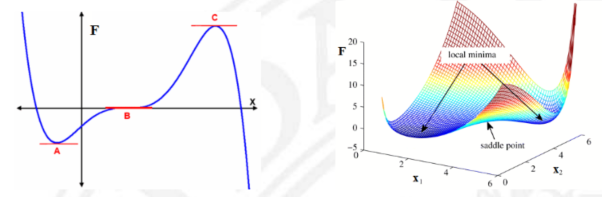
\includegraphics[width=10cm]{Imagenes/Captura de pantalla 2024-03-09 153948.png}
                \caption{comparación de puntos estacionarios en 1 y 2 dimensiones.}
                \centering
            \end{figure}
        \end{frame}
    \subsection{Optimización en una dimensión}
        \begin{frame}{Optimización en una dimensión}
            \begin{figure}[h]
                \centering
                \captionsetup{justification=centering}
                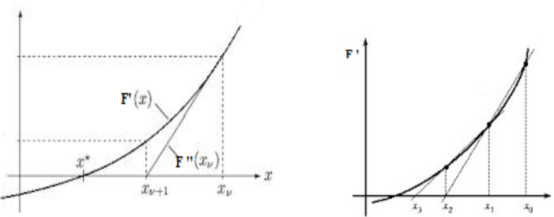
\includegraphics[width=10cm]{Imagenes/Captura de pantalla 2024-03-09 152833.png}
                \caption{Comparación entre el método de Newton Y
                el método de la secante}
                \centering
            \end{figure}
        \end{frame}
    \subsection{Métodos locales para optimización no restringida}
        \begin{frame}{Métodos locales para optimización no restringida}
            \begin{itemize}
                \item Método de Newton para dimensiones mayores
                %Se utiliza el Hessiano
                \item Métodos Quasi-Newtonianos.
                %Se aproxima el Hessiano
                \item Métodos Quasi-Newtonianos para sistemas a gran escala.
                %Se evita usar matrices grandes producidas por el Hessiano
                %Considerando que los resultados de algunos productos
                %son o vectores o escalares se almacenan dichos valores
                %en vez de almacenar los Hessianos producidos en cada iteración.
                %utilizando el método conocido como BFGS Broyden–Fletcher–Goldfarb–Shanno
                \item Métodos de descenso
                %Método aproximado que utiliza un vector normalizado
                %para acercarse al mínimo de la función
                \item Métodos de descenso paso a paso.
                
                \item Métodos de la gradiente conjugada.
            \end{itemize}
        \end{frame}
    \subsection{Combinación de métodos}
        \begin{frame}{Combinación de métodos}
            \begin{figure}[h]
                \centering
                \captionsetup{justification=centering}
                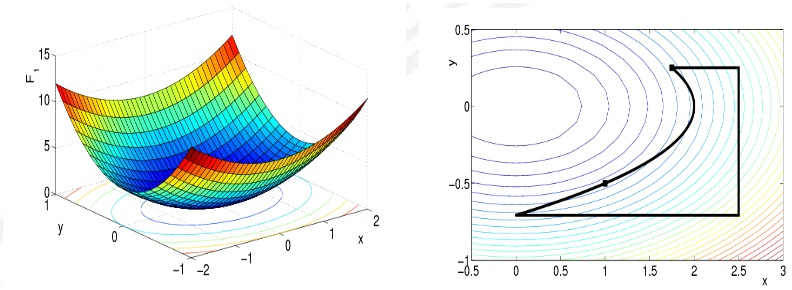
\includegraphics[width=10cm]{Imagenes/Funciones convexas.jpg}
                \caption{Función analizada con los diferentes métodos}
                \centering
            \end{figure}
        \end{frame}
        \begin{frame}{Combinación de métodos}
            \begin{figure}[h]
                \centering
                \captionsetup{justification=centering}
                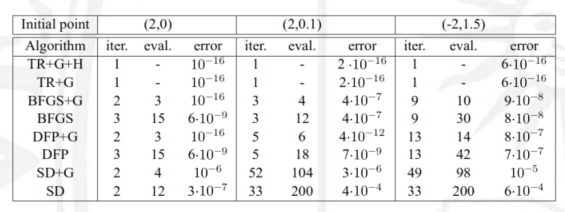
\includegraphics[width=10cm]{Imagenes/Captura de pantalla 2024-03-09 155904.png}
                \caption{Tiempos de respuesta de los diferentes métodos en matlab}
                \centering
            \end{figure}
        \end{frame}
    \subsection{Optimización restringida}
        \begin{frame}{Optimización restringida}
            \begin{figure}[h]
                \centering
                \captionsetup{justification=centering}
                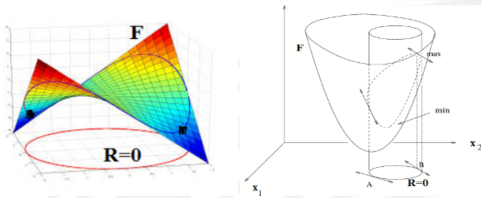
\includegraphics[width=10cm]{Imagenes/Captura de pantalla 2024-03-09 160319.png}
                \caption{Ejemplo de optimización restringida}
                \centering
            \end{figure}
        \end{frame}
        \begin{frame}{Optimización restringida}
\begin{itemize}
    \item Métodos de penalidad, funciones barrera y variables sueltas
    \item Multiplicadores de Lagrange y condiciones KKT
    \item Funciones lagrangianas
    \item Método de Newton y programación cuadrática
\end{itemize}
        \end{frame}
        \begin{frame}{Optimización restringida}
            \begin{figure}[h]
                \centering
                \captionsetup{justification=centering}
                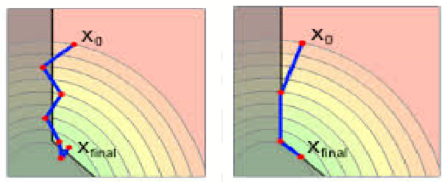
\includegraphics[width=10cm]{Imagenes/Captura de pantalla 2024-03-09 153248.png}
                \caption{comparación de métodos de penalidad y métodos de conjuntos activos 
                aproximándose a un mínimo local en el extremo}
                \centering
            \end{figure}
        \end{frame}
    \subsection{últimas observaciones sobre los métodos tipo gradiente}
        \begin{frame}
                
        \end{frame}
%\footcite{Car12}
%\begin{frame}[noframenumbering,plain,allowframebreaks]{Referencias}
%    \printbibliography[heading=none]
%\end{frame}

\end{document}
